\section{Diseño}
En esta sección tiene como propósito documentar el proceso de desarrollo de parte del equipo encargado del desarrollo del módulo de Curriculum, debido a que el módulo de Curriculum es un proyecto y dicho proyecto está dividido en varias épicas utilizadas para implementar las exigencias de los clientes de Estados Unidos.

Una épica se encuentra dividida en varias historias de usuario, donde las historias de usuario tienen el propósito de entregar valores de negocio al cliente en un periodo máximo de 2 semanas. Estas historias de usuario pueden ser a la vez divididas buscando la simplicidad de las historias donde se busca que se encuentren de ser posible bajo el estándar INVEST (independientes, negociables, valoradas, estimables, pequeñas, verificables) de la metodología ágil.

Como una épica consiste en un conjunto de historias de usuario que los desarrolladores podían terminar en un sprint, esta épica tiene una variedad de historias de usuario. Cada historia de usuario está compuesta de sub-tareas que tiene como propósito facilitar al desarrollador recordar cuales eran algunas labores pendientes a la hora de desarrollar la historia. Cada tarea debía tener un encargado, pero eso no significaba que esa persona debía hacer sola la implementación.

\begin{figure}[H]
\centering
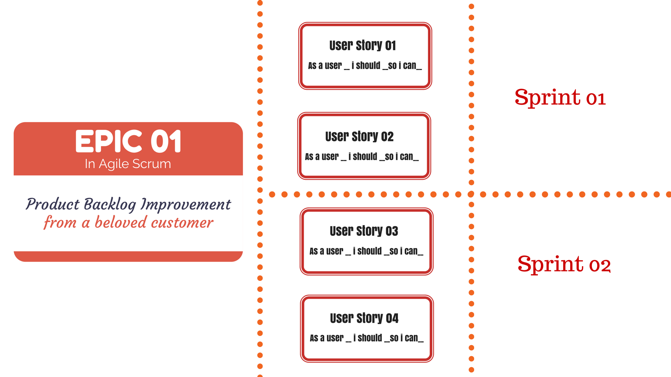
\includegraphics[width=125mm,scale=1]{Figuras/proceso/epic}
\caption{HACER MI PROPIO DIAGRAMA}
  \label{epic}
\end{figure}

El PO (siglas en inglés que significa dueño o responsable del producto) se encarga de la creación de épicas e historias de usuario, en caso de que la historia sea muy grande para terminar en un solo sprint se vuelve a partir en historias más pequeñas. 

Cada sprint consta de 2 semanas de trabajo, donde los desarrolladores como equipo se comprometen a entregar cierto valor de negocio que ellos estiman poder terminar en dicho periodo. En caso de que el equipo presienta que la totalidad de historias no van a poder ser entregadas antes de que termine el periodo se pasa al siguiente sprint o se achica la historia con los criterios de aceptación y los criterios de aceptación restantes se agregan en otra historia de usuario para el siguiente sprint.

Cada equipo tiene un líder, donde cada líder tiene como rol ser la brecha que une al PO con los desarrolladores. El PO se reúne con el líder de cada equipo para verificar las prioridades de las historias de usuario que están pendientes en el backlog. 

Al terminar una historia de usuario, se deben cumplir los criterios de aceptación para que sea considerada como realizada y los clientes puedan empezar a utilizar las nuevas características del sistema. En caso de que la historia no consiga cumplir los criterios de aceptación correspondientes se considera que la historia no está terminada y que debe mantenerse abierta o se debe volver a abrir en caso de que fue cerrada. Estos criterios de aceptación se verifican primeramente por los mismos desarrolladores antes de cambiar el estado de la historia a resuelto o “done”. Luego, la historia pasa a ser verificada por un grupo experto en dominios de didáctica en universidades norteamericanas incluyendo a un PhD en educación. Si en las dos partes la historia es aprobada, entonces pasa al estado de realizado. 

Cualquier otro problema o error de código que tenga la nueva característica se debe crear un ticket de bug especificando como reproducir el problema y el comportamiento esperado. En caso de no poder reproducir este comportamiento se pide más información al respecto o pasa al estado de “won’t do” en caso de que el comportamiento ya no se pueda reproducir.

Esta sección va a consistir en explicar cómo se dividieron algunas épicas.


\subsection{SCRUM}
Scrum es un proceso en el que se aplican de manera regular un conjunto de buenas prácticas para trabajar colaborativamente, en equipo, y obtener el mejor resultado posible de un proyecto. Estas prácticas se apoyan unas a otras y su selección tiene origen en un estudio de la manera de trabajar de equipos altamente productivos.

En Scrum se realizan entregas parciales y regulares del producto final, priorizadas por el beneficio que aportan al receptor del proyecto. Por ello, Scrum está especialmente indicado para proyectos en entornos complejos, donde se necesita obtener resultados pronto, donde los requisitos son cambiantes o poco definidos, donde la innovación, la competitividad, la flexibilidad la productividad son fundamentales.

Scrum también se utiliza para resolver situaciones en que no se está entregando al cliente lo que necesita, cuando las entregas se alargan demasiado, los costes se disparan o la calidad no es aceptable, cuando se necesita capacidad de reacción ante la competencia, cuando la moral de los equipos es baja y la rotación alta, cuando es necesario identificar y solucionar ineficiencias sistemáticamente o cuando se quiere trabajar utilizando un proceso especializado en el desarrollo de producto. 

\subsection{Proceso}
En Scrum un proyecto se ejecuta en bloques temporales cortos y fijos (sprints o iteraciones que normalmente son de 2 semanas, aunque en algunos equipos son de 3 y hasta 4 semanas, límite máximo de feedback y reflexión). Cada iteración tiene que proporcionar un resultado completo, un incremento de producto final que sea susceptible de ser entregado con el mínimo esfuerzo al cliente cuando lo solicite.

El proceso parte de la lista de objetivos o requisitos priorizada del producto, que actúa como plan del proyecto. En esta lista el cliente prioriza los objetivos balanceando el valor que le aportan respecto a su coste y quedan repartidos en sprints y entregas.

\begin{figure}[H]
\centering
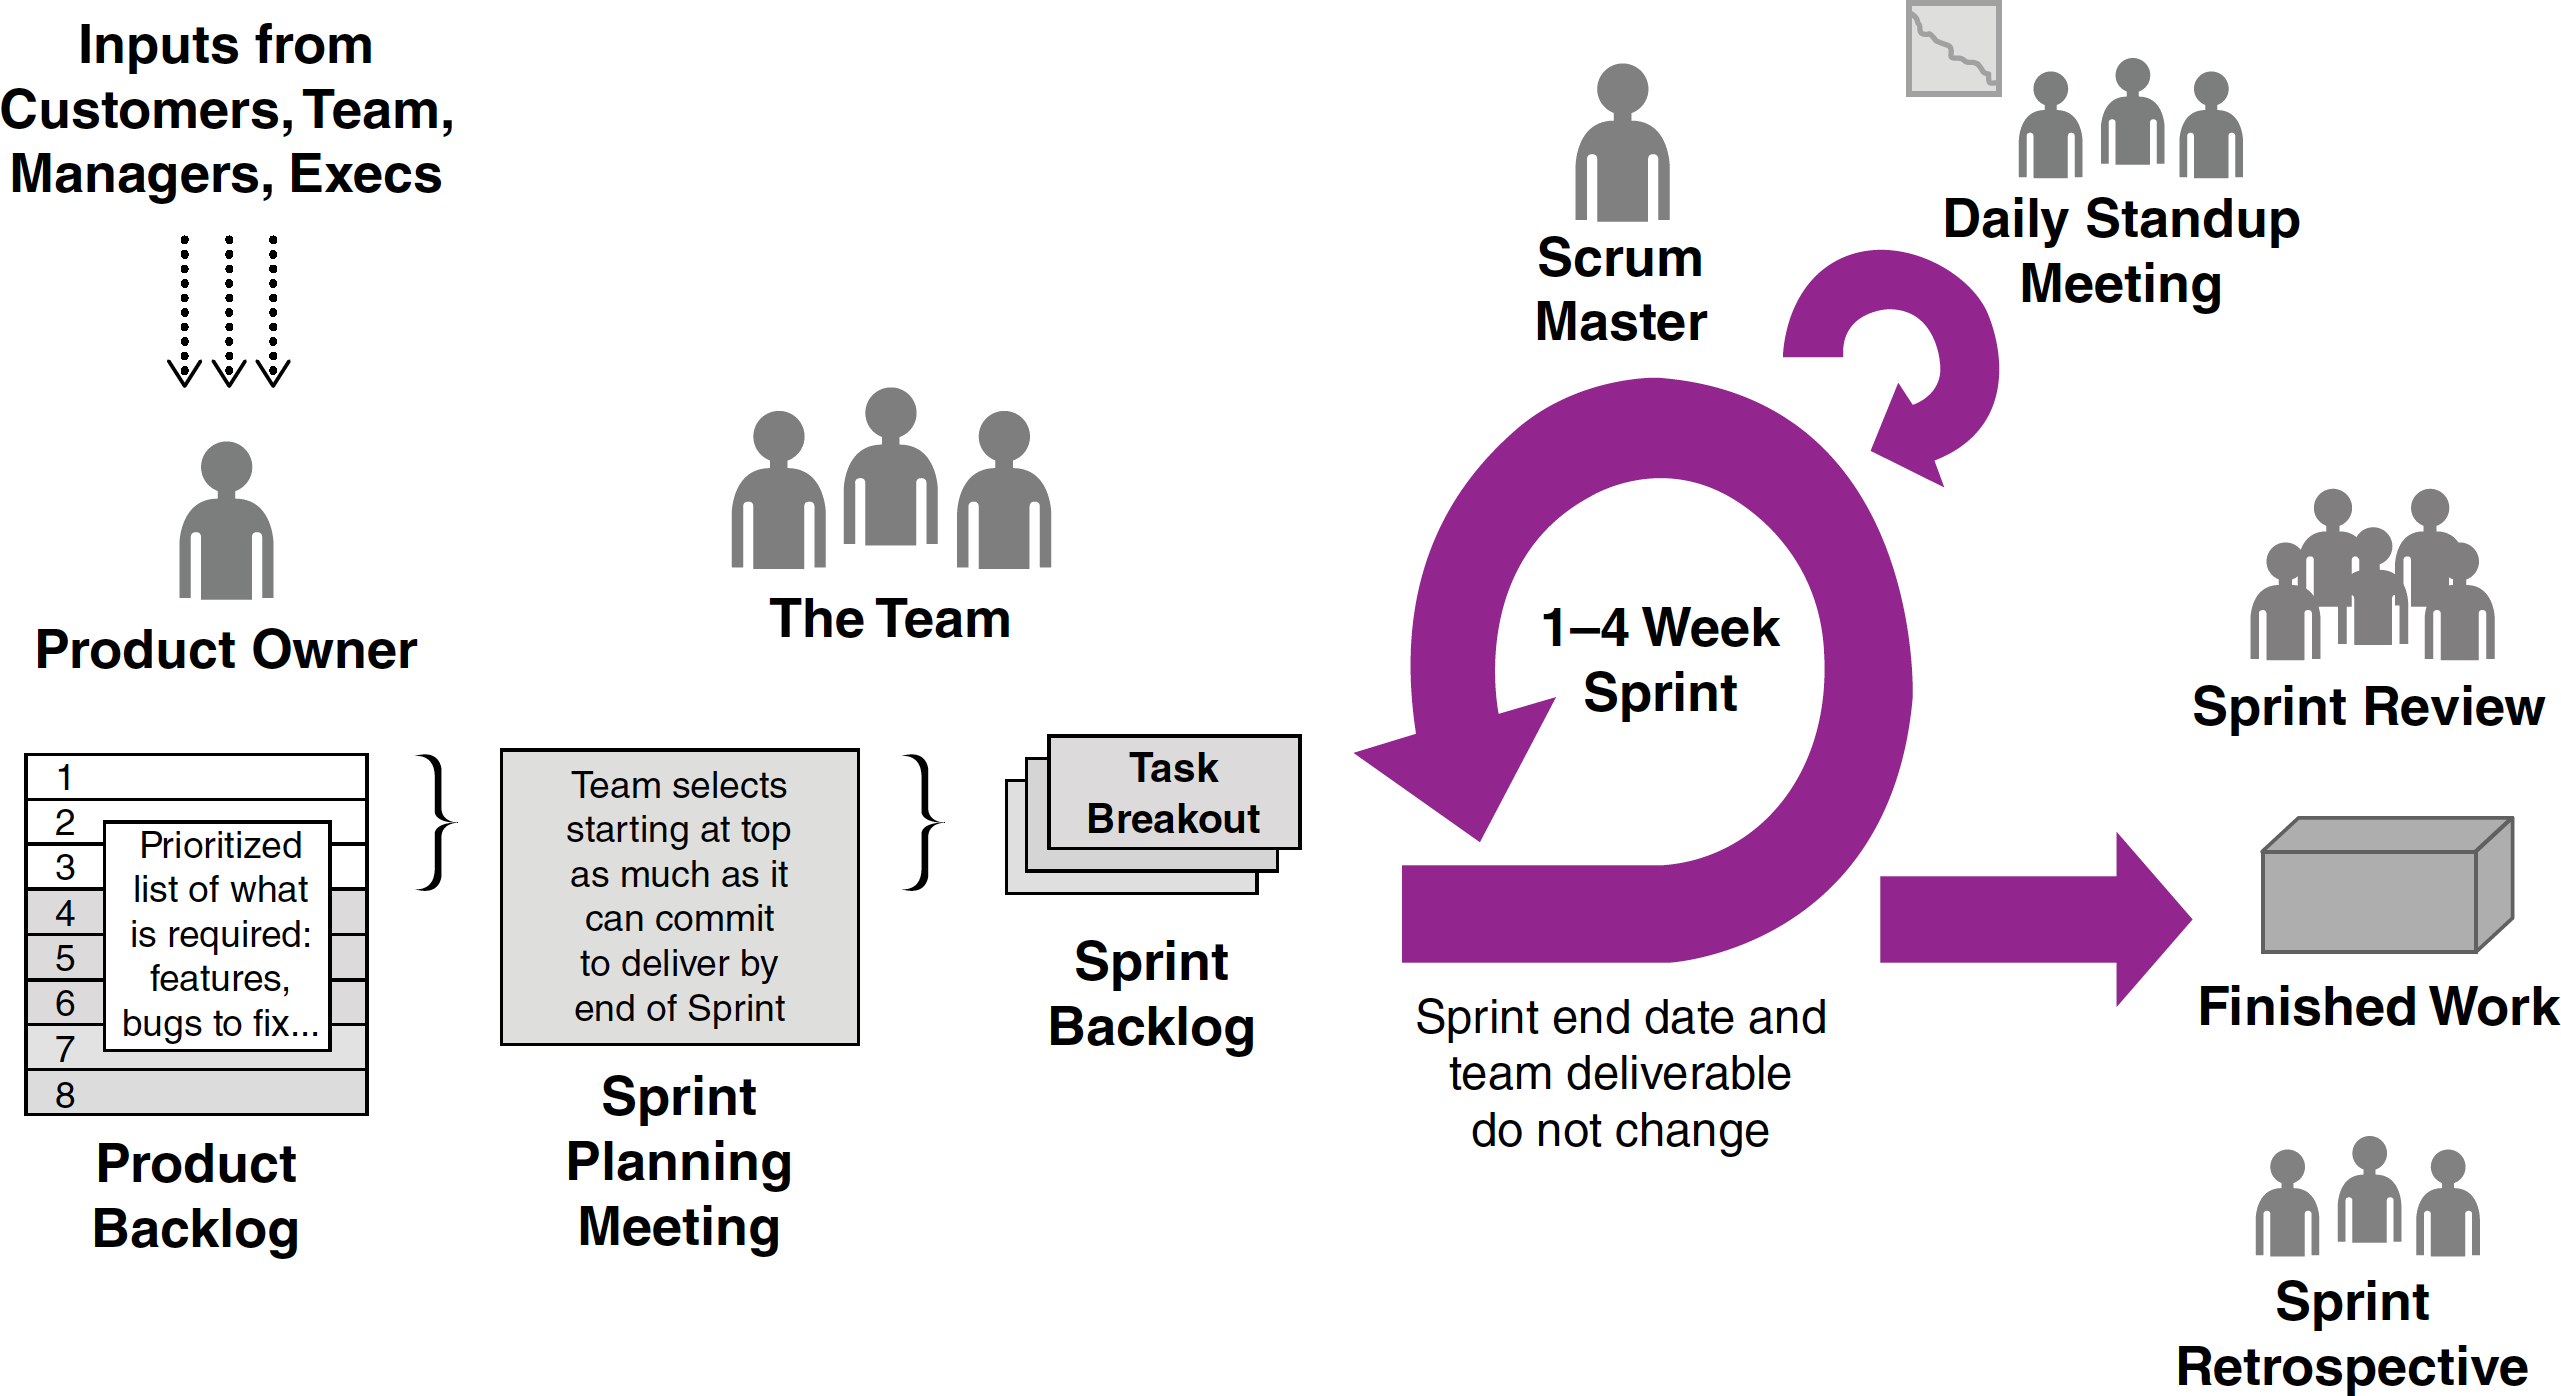
\includegraphics[width=125mm,scale=1]{Figuras/flujo_scrum}
\caption{Flujo de la técnica SCRUM.}
  \label{flujo_scrum}
\end{figure}

\subsection{Planificación de iteraciones}
El primer día de la iteración se realiza la reunión de planificación de la iteración. Tiene dos partes:
\begin{itemize}
    \item \textbf{Selección de requisitos} (4 horas máximo) – El cliente presenta al equipo la lista de requisitos priorizada del producto o proyecto. El equipo pregunta al cliente las dudas que surgen y selecciona los requisitos más prioritarios que se compromete a completar en la iteración o sprint, de manera que puedan ser entregados si el cliente lo solicita.
    \item \textbf{Planificación de la iteración o sprint} (4 horas máximo) – El equipo elabora la lista de tareas de la iteración necesarias para desarrollar los requisitos a que se ha comprometido. La estimación de esfuerzo se hace de manera conjunta y los miembros del equipo se auto-asignan las tareas.
\end{itemize}

\subsection{Ejecución del Sprint}
Cada día el equipo realiza una reunión diaria (15 minutos aproximadamente). Cada miembro del equipo inspecciona el trabajo que el resto está realizando (dependencias entre tareas, progreso hacia el objetivo de la iteración, obstáculos que pueden impedir este objetivo) para poder hacer las adaptaciones necesarias que permitan cumplir con el compromiso adquirido. En la reunión cada miembro del equipo responde a tres preguntas:
\begin{itemize}
    \item ¿Qué he hecho desde la última reunión diaria?
    \item ¿Qué voy a hacer a partir de este momento?
    \item ¿Qué impedimentos tengo o voy a tener?
\end{itemize}
Durante la iteración el Scrum Master se encarga de que el equipo pueda cumplir con su compromiso y de que no se merme su productividad. Además, elimina los obstáculos que el equipo no puede resolver por sí mismo.

Durante el sprint, el cliente junto con el equipo refina la lista de requisitos (para prepararlos para los siguientes sprints) y, si es necesario, cambian o vuelven a planificar los objetivos del proyecto para maximizar la utilidad de lo que se desarrolla y el retorno de inversión.

\subsection{Inspección y adaptación}
El último día de la iteración se realiza la reunión de revisión del sprint. Tiene dos partes:
\begin{itemize}
    \item \textbf{Demostración} (3 horas aproximadamente) – El equipo presenta al cliente los requisitos completados en la iteración, en forma de incremento de producto preparado para ser entregado con el mínimo esfuerzo. En función de los resultados mostrados y de los cambios que haya habido en el contexto del proyecto, el cliente realiza las adaptaciones necesarias de manera objetiva, ya desde la primera iteración, volviendo a planificar el proyecto.
    \item \textbf{Retrospectiva} (1 hora) - El equipo analiza cómo ha sido su manera de trabajar y cuáles son los problemas que podrían impedirle progresar adecuadamente, mejorando de manera continua su productividad. El Facilitador se encargará de ir eliminando los obstáculos identificados.
\end{itemize}